\documentclass{beamer}
\newcommand{\myfont}{\rmfamily\normalsize\upshape\mdseries}
\newcommand{\degree}{^\circ}
\title{\sffamily Midterm Rivew -  Part II}
\subtitle{\textbf{Mathematical Logic and Algebraic Structure}\\Logic, Induction, Group Theory}
\institute[UM-SJTU JI]{University of Michigan-Shanghai Jiao Tong University Joint Institute}
\author{HamHam}
\usepackage{graphicx}
\usepackage{picinpar}
\usepackage{indentfirst}
\usepackage{chemformula}
\usepackage{geometry}
\usepackage{subfigure}
\usepackage{appendix}
\usepackage{amsfonts}
\usepackage{enumerate}
\usepackage{float}
\usepackage{geometry}
\usepackage{latexsym}
\usepackage{listings}
\usepackage{multicol,multirow,multido}
\usepackage{tabularx}
\usepackage{ulem}
\usepackage{tikz}
\usepackage{xcolor}
\usepackage{cite}
\usepackage{setspace}
\usepackage{hyperref}
\usepackage{textpos}
\usepackage{booktabs}
\usepackage{diagbox}
\usepackage{listings}
\usepackage{graphics}
\usepackage{upgreek}
\usepackage{JI_MathCourse_Notations}
\usepackage{mathrsfs}
\usepackage[final]{pdfpages}
%\usepackage{boondox-cal}
\usepackage{dutchcal}
\usepackage{colortbl}
%\usepackage{ctex} %插入中文
%\ctexset{today=old}

\newcommand{\mydef}[1]{\sffamily\blue{#1}\myfont\\} %for define
\newcommand{\mysol}{\yellow{Solution:}\\}
\usetheme[dove]{Boadilla}
\usecolortheme{dolphin}
\useoutertheme{miniframes}
\begin{document}
    \usebackgroundtemplate{\tikz\node[opacity=0.25]{
    
\includegraphics[width=\paperwidth,
    height=\paperheight]{hamster.jpg}
    };}
\begin{titlepage}
    \begin{center}
        VE203 - Discrete Mathmatics 
    \end{center}
\end{titlepage}
\myfont
\newcommand{\binomial}[2]{\begin{pmatrix} {#1}\\{#2}	\end{pmatrix}}
\newcommand{\green}[1]{\textcolor[rgb]{0.3,0.6,0}{#1}}
\definecolor{mygray}{gray}{.9}
\section{Propositional Logic}
\begin{frame}
    \frametitle{Propositional Logic}
    \hh A \green{proposition} or \green{statement} is a declarative sentence that is either 
    \textbf{true} or \textbf{false}, but not both.
    \\ 
    \hh Four binary connectives  $\wedge$ (conjunction), $\vee$ (disjunction), $\to$ (implication), and $\leftrightarrow$ (biconditional).
    \\ \vv
    \begin{minipage}{\textwidth}
        \begin{minipage}[t]{0.45\textwidth}
            \centering
            \begin{tabular}{ccc}
                \hline
                $p$ & $q$ & $p \to q$ \\ \hline
                 0  &  0  &     1     \\
                 0  &  1  &     1     \\
                 \rowcolor{mygray} 1  &  0  &     0     \\
                 1  &  1  &     1     \\ \hline
            \end{tabular}
        \end{minipage}
        \begin{minipage}[t]{0.45\textwidth}
            \centering
            \begin{tabular}{ccc}
                \hline
                $p$ & $q$ & $p \leftrightarrow q$ \\ \hline
                 0  &  0  &           1           \\
                 0  &  1  &           0           \\
                 1  &  0  &           0           \\
                 1  &  1  &           1           \\ \hline
            \end{tabular}
        \end{minipage}
    \end{minipage}	
    \vv
    \par \phantom{jijiijij}$(p \to q) \Leftrightarrow (\neg p \vee q)$ \phantom{jijijijijijiji}$(p \leftrightarrow q) \Leftrightarrow ((p \to q) \wedge (q \to p))$ 
\end{frame}
\begin{frame}
    \frametitle{Important Tautologies}
    \par \blue{De-Morgan rules}
	$$
	\neg(p \vee q) \Leftrightarrow(\neg p) \wedge(\neg q), \quad \neg(p \wedge q) \Leftrightarrow(\neg p) \vee(\neg q) .
	$$
	\par \phantom{ji}
	\par The \blue{contrapositive} of $p \rightarrow q$ :
	$$
	(p \rightarrow q) \Leftrightarrow(\neg p \rightarrow \neg q),
	$$
	Proof by \blue{contradiction}:
    $$
    (p \rightarrow q) \LRarrow (p \wedge \neg q) \rarrow 0
    $$
\end{frame}
\begin{frame}
    \frametitle{Predicates}
    \mydef{Definition}
    \par \hh A function $P: X \to \{\top, \perp \}$ is called a \textbf{predicate} on its domain $X$. 
    \\\vv
    \par \hh It is a declarative sentence involving variables, \textit{i.e.}, a statement involving variables such that when the variables a substituted with appropriate individuals we obtain a \textbf{proposition}.
    \\\vv
    \begin{itemize}
        \item \textbf{Predicate:} $P(x): x>1$;
        \item \textbf{Proposition:} $P(0): 0>1$ (false); $P(2): 2>1$ (true).
    \end{itemize}
\end{frame}
\begin{frame}
    \frametitle{Exercise}
    1. Given logical variables $p$ and $q$, which of the following are tautologies?
    \begin{itemize}
        \item[(A)] $p\wedge \neg p$
        \item[(B)] $((p\rarrow q )\wedge \neg q )\rarrow \neg q$
        \item[(C)] $p \vee q \rarrow p$
        \item[(D)] $p \rarrow(p \wedge q)$  
    \end{itemize}
    \vv 
    \yellow{Answer:} \textcolor[cmyk]{0.01,0.01,0.01,0.01}{A\,B}
    \\ \vv 
    \textit{Comment.} There is no choice question in this exam.
\end{frame}
\section{Induction}
\begin{frame}
    \frametitle{Induction}
    \hh An argument by \textbf{strong} induction that shows that a property $A(n)$ holds for all $n \in \mathbb{N}$  with $n \geqslant n_0 $ proceeds as follows:
		\begin{enumerate}
			\item Show that $A(n_0)$ holds;
			\item Show that for all $n \geqslant n_0 $, if $A(n)$ holds, then $A(n + 1)$ holds;\\
			$\to$ ``Assuming the statement is true for $n$, we now show that it is true for $n + 1$''
			\item Conclude that for all $n \in \mathbb{N}$ with $n \geqslant n_0 $, $A(n)$ holds.
		\end{enumerate}
    \begin{block}{Terminology}
        \begin{itemize}
            \item Type-I \& Type-II Induction
            \item IH - Induction Hypothesis
        \end{itemize}
    \end{block}
\end{frame}
\begin{frame}
    \frametitle{Interesting Exercise}
    \hh \textbf{If you think the following problem is too hard for you, just ignore it.}\\
    \vv 
    \hh There is a board which is divided into $8 \times 8$ small lattices. One of the
    lattice is broken (its location is unknown). Prove that we can always
    place 21 small ``L'' cards on this board. Note that a ``L'' card consists of
    three lattices in the form of ``L''.
    \\ 
    \vs{2em} 
    \hh \textit{Hint.} Generalize $8$ to $n$ wouldn't work. Is there another way to
    generalize the problem?

\end{frame}
\begin{frame}
    \frametitle{Exercise}
    2. Given a poset $(P, \leq)$. Use induction to show that every finite non-empty set
    $Q \subset P$ admits a minimal element with respect to $\leq$.
    
    

\end{frame}
\begin{frame}{Exercise}
    \par We define the set $S \subset \mathbb{Z}^2$ by the following properties
    \begin{itemize}
        \item $(3,5) \in S$
        \item $(x,y) \in S \Rightarrow (x + 2,y) \in S$
        \item $(x,y) \in S \Rightarrow (-x,y) \in S$
        \item $(x,y) \in S \Rightarrow (y,x) \in S$
    \end{itemize}
    \par Show that $S = T$, where
    $$
    T=\left\{(x, y) \in \mathbb{Z}^{2}: \underset{m, n \in \mathbb{Z}}\exists(x, y)=(2 m+1,2 n+1)\right\}.
    $$
\end{frame}
\section{Addictive Groups}

\begin{frame}{Group}
    \hh A \textbf{group} is a pair $(G, \cdot)$, where $G$ is a set, and $\cdot : G \times G \to G$ is a law of composition that has the following properties:
    \begin{itemize}
        \item The law of composition is \textbf{associative}: $(a \cdot b) \cdot c = a \cdot (b \cdot c)$ for all $a, b, c \in G$;
        \item $G$ contains an \textbf{identity} element 1, such that $1 \cdot a = a \cdot 1 = a$ for all $a \in G$;
        \item Every element $a \in G$ has an \textbf{inverse}, an element $b$ such that $a \cdot b = b \cdot a = 1$.
    \end{itemize}
    \par \phantom{ji}
    \par 
    \hh An \textbf{abelian group} is a group whose law of composition is \textbf{commutative} $(a \cdot b = b \cdot a)$. 
\end{frame}
\begin{frame}{Subgroup}
    \par A subset $H$ of a group $G$ is a subgroup if it has the following properties:
    \begin{itemize}
        \item Closure: If $a, b \in H$, then $a \cdot b \in H$;
        \item Identity: $\mathbf{1_G} \in H$;
        \item Inverses: If $a \in H$, then $\mathbf{a^{-1}_G} \in H$.
    \end{itemize}
    \begin{block}{Question}
        \hh How to prove/disprove $H$ is a subgroup of $G$?
    \end{block}
\end{frame}
\begin{frame}{Subgroup of $(\mathbb{Z}, +)$}
    \par For $a \in \mathbb{Z}$, a subgroup of $(\mathbb{Z}, +)$ is given by integers divisible by $a$ as,
    $$
    a \mathbb{Z}=\{n \in \mathbb{Z} \mid n=k a \text { for some } k \in \mathbb{Z}\}.
    $$
    \par \phantom{ji}
    \par Given $a, b \in \mathbb{Z}$, then the subgroup $S$ generated by $a$ and $b$, denoted by
    $$
    S=\mathbb{Z} a+\mathbb{Z} b=\{n \in \mathbb{Z} \mid n=r a+s b \text { for some integers } r, s\}
    $$
    \par It is also the smallest subgroup that contains both $a$ and $b$.
\end{frame}
\begin{frame}{Exercise}
    \par 3. Let $S$ be a subgroup of the additive group $(\mathbb{Z}, +)$. Prove that 
    \begin{itemize}
        \item either $S$ is the trivial subgroup $(\{0\}, +)$,
        \item or it has the form $a\mathbb{Z}$, where $a$ is the smallest positive integer in $S$.
    \end{itemize}
\end{frame}

\section{Cyclic Groups}
\begin{frame}{Cyclic Group}
    \hh A group is cyclic if it can be generated by a single element.
    \hh The cyclic subgroup generated by $g$ is
    $$
    \left\langle g \right\rangle = \{g^k \mid k \in \mathbb{Z}\}.
    $$
    \hh Let $G$ be a group, $g \in G$. The \green{order} of $g$ is the smallest natural integer $n$ such that $g^n = 1$. If there is no positive integer $n$ such that $g^n = 1 $, then $g$ has infinite order.
    \par \phantom{ji}
    \hh A group $G$ is cyclic if $G = \left\langle g \right\rangle$ for some $g \in G$. $g$ is a generator of $\left\langle g \right\rangle$.
    \begin{block}{Notations}
        \hh Oder of a element vs. Order of a group: $|g| \quad |\<g\>| \quad |G|$
    \end{block}
\end{frame}
\begin{frame}{Exercise}
    4. Let $(G, \cdot)$ be a finite. Prove that if $G$ is cyclic and the order of $G$ is even, then $G$
has exactly one element of order $2$.

\end{frame}
\begin{frame}{Symmetric Group}
    \hh Given $n \in \mathbb{N} \backslash \{0\}$, we have the following symmetric group of degree $n$, $S_{n} =\{\text {All permutations on } n \text { letters/numbers}\}$.
    Note that it is a finite group of order $n!$.
    \par 
    \vs{1em}
    \hh The permutation does not satisfy the law of communication. 
    However, if two permutations $\sigma$ and $\tau$ are \textbf{disjoint}, we have $\sigma \tau = \tau \sigma$.
    \par 
    \vv
    \hh The order of operations is \textbf{from right to left}.
    \end{frame}
\begin{frame}{Symmetric Group}
    \hh A permutation of the form $(ab)$ where $a \neq b$ is  a \textbf{transposition}.
    \par \vv
    \hh A permutation that can be expressed as a product of an even/odd number of \textbf{transpositions} is called an even/odd permutation. 
    \par \vv
    \hh The set of even permutations in $S_n$ forms a subgroup of $S_n$, denoted $A_n$, is called the alternating group of degree $n$.  $|A_n| = n!/2$ for $n > 1
    $.
\end{frame}

\begin{frame}{Exercise}
    5. Prove that for $n \geqslant 3$, every element of $A_n$ is a product of 3-cycles.
\end{frame}
\section{Homomorphism}
\begin{frame}{Homomorphism}
	\hh Given groups $G,G'$, a homomorphism is a map $f : G \to G\,'$ such that for all $x, y \in G$,
     $$f \(xy\) = f \(x\)f \(y\)$$	
	\par Two important properties:  
	\begin{itemize}
		\item  $f\left(1_{G}\right)=1_{G^{\prime}}$
		\item $f\left(a^{-1}\right)=f\(a\)^{-1}$
	\end{itemize}
	\end{frame}
\begin{frame}{Image and Kernel}
	\hh The \green{image} of a homomorphism $f : G \to G\,'$, often denoted by im$f$, or $f\(G\)$, is simply the image of as a map of sets:
	$$
	\operatorname{im} f=\left\{x \in G\,^{\prime} \mid x=f\(a\) \text { for some } a \in G\right\}.
	$$
    \\
	\vv 
	\hh The \green{kernel} of $f$ , denoted by ker$f$, is the set of elements of $G$ that are	mapped to the identity in $G\,'$:
	$$
	\operatorname{ker} f=\left\{a \in G \mid f\(a\)=1_{G^{\prime}}\right\}.
	$$
\end{frame}
\begin{frame}{isomorphism}
	\hh Given groups $G$ and $G\,'$, an isomorphism $f : G \to G\,'$ is a \textbf{bijective} group homomorphism, 
    \textit{i.e.}, a bijection $f \(xy\) = f \(x\) f \(y\)$ for all $x, y \in G$.
	\\ \vv \hh 
	Check if a \textbf{homomorphism} $f : G \to G\,'$ is an isomorphism: verify ker$f = \{1_G\}$ (injection) and im$f = G\,'$ (bijection).
\end{frame}
\begin{frame}
    \frametitle{Exericse}
    6. Given group $G$ and $a \in G$ a fixed element, define $\gamma_a : G \to G$, by $\gamma_a \(x\) = a x a^{-1}$.
    \begin{itemize}
        \item[(1)] Show that $\gamma_a$ is a isomorphism.
        \item[(2)] If $a,b \in G$, show that $\gamma_a \circ \gamma_b = \gamma_{ab}$ 
    \end{itemize}
\end{frame}
\begin{frame}{Cosets}
    \hh Given a group $G$, if $H$ is a subgroup pf $G$ and $a \in G$, 
    then a \green{left coset} of $H$ in $G$ can be defined as
    $$
    a H=\{g \in G \mid g=ah \text { for some } h \in H\}
    $$
    \\ 
    \hh The number of left cosets of a subgroup is the \green{index} of $H$ in $G$ $[G : H]$ (which could be infinite if $|G| = \infty$). All left cosets $aH$ of a subgroup $H$ of a group $G$ have the same order.
    \begin{itemize}
        \item[-]Counting formula: $|G| = |H| \cdot [G : H].$
        \item[-]Lagrange's Theorem: Let $H$ be a subgroup of a finite group $G$. The order of $H$ divides the order of $G$.
    \end{itemize}
    \par 
\end{frame}
\begin{frame}
    \frametitle{Exericse}
    7. Prove Lagrange's Theorem.
    \vs{15em}

\end{frame}
\begin{frame}{Normal Subgroup}
    \hh Given group $G$, and $a, g \in G$, the element $gag^{-1} \in G$ is called the
    \green{conjugate} of a by $g$.
    \\ \vv \hh
     A subgroup $N$ of $G$ is a normal subgroup, denoted by $N \unlhd G$, if for all $a \in N$ and $g \in G$, $gag^{-1} \in N$. 
    \\ \vv \hh 
     $N \unlhd G \ \equiv \ gNg^{-1} = H$ for all $g \in G \ \equiv \ gN = Ng$ for all $g$.
\end{frame}
\begin{frame}
    \frametitle{Exercise}
    8. Let $G$ be a group and $N \unlhd G$ be a normal 
    subgroup. We define a binary operation on $G/N$ as follows: 
    for $aN, bN \in G/N$ we set $$(aN)(bN) = abN.$$ 
    Show that the quotient group $G/N$ exists.
	\par \vs{2em}
    Note: $G / N := \{aN \mid a \in G \}$  %\left{a N \mid a \in G \right}$
\end{frame}
\section{End}
\begin{frame}
    \frametitle{Final Remarks}
    Hmm... Here's something I want to say:
    \\ \vv 
    \begin{itemize}
        \item no choice question in the exam.
        \item Take a look at last semester's mid1 \& mid2 paper.
        \item Take quiz part I \& II.
        \item Look at our OH feedbacks and questions on piazza.
        \item \red{DO GET UP!} This is an early-eight exam. 
        It's better to have breakfast first. 
            \begin{itemize}
                \item Exam Time: 8:00 - 9:40
                \item Submit Time: 9:40 - 9:45
            \end{itemize}
        \item Be confident! The exam will be easy!
    \end{itemize}
\end{frame}
\usebackgroundtemplate{}
\begin{frame}
    \frametitle{}
    \usebackgroundtemplate{}
    \centering
    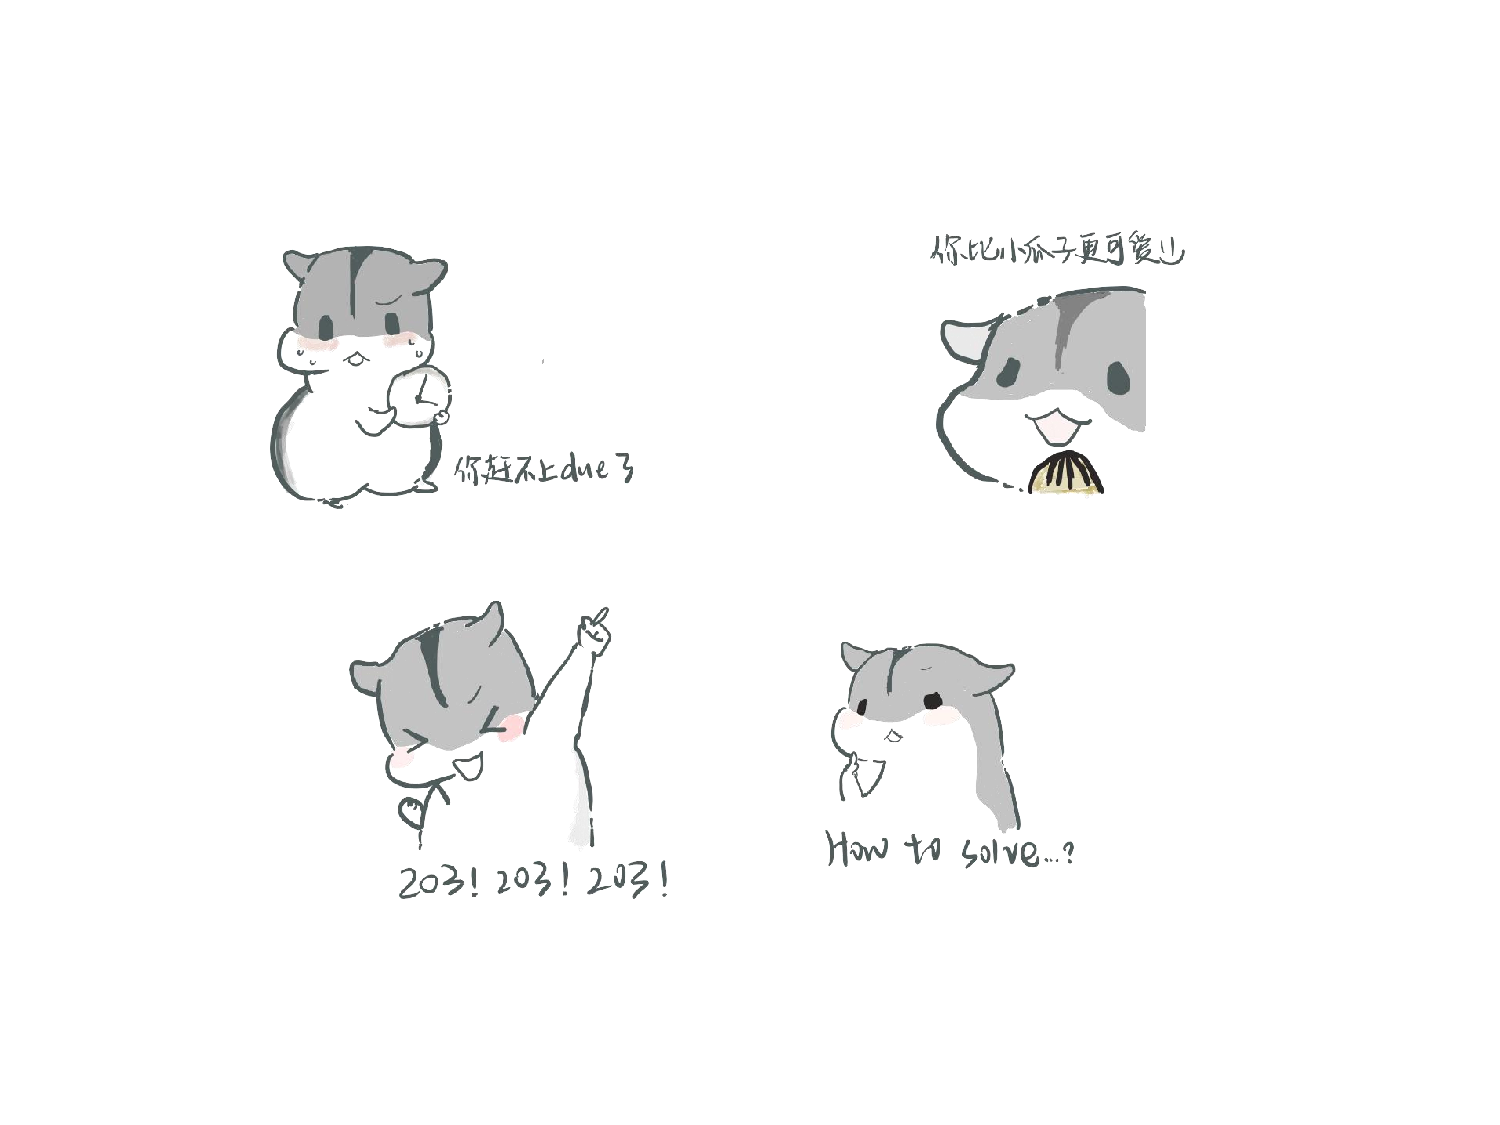
\includepdf[nup=1x1,scale=1.4]{new.pdf}
    \textcolor[rgb]{0.3,0.3,0.3}{\textbf{\huge{$\mathcal{Good~Luck~For~Your~Exam}$!}}}
\end{frame}
\usebackgroundtemplate{\tikz\node[opacity=0.25]{
    
\includegraphics[width=\paperwidth,
    height=\paperheight]{hamster.jpg}
    };}
\begin{frame}
    \frametitle{Reference}
    \begin{itemize}
        \item Exercises from Zach's Practice Exam.
        \item Content from Ve203-2021-fall Mid\_1 \& Mid\_2 RC by Zhao Jiayuan.
        \item Exericses from Ve203-2021-fall Mid\_1 \& Mid\_2 Exam.
        \item Cute paintings of Hamham from Wang Ruizhe.
        \item Exercises from Ve203-2020-fall TA Zhang Gutao.
        %\item Exercises from 2019-Fall-Ve203 TA Yan Xinyu.
        %\item Contents from 2021-Fall Mid\_2\_RC by Xue Runze.
        %\item Yan Shijian, etc. \textit{Basic Number Theory},
        %fourth edition. Beijing: Higher Education Press, 2020.5 print.
    \end{itemize}
\end{frame}
\end{document}